% Drawing a graph
% Author: Stefan Kottwitz
% https://www.packtpub.com/hardware-and-creative/latex-cookbook
\documentclass[border=10pt]{standalone}
\usepackage{tkz-graph}

\tikzset{
  LabelStyle/.style = { rectangle, rounded corners, draw,
                       font = \bfseries },
  EdgeStyle/.append style = {->} }
\thispagestyle{empty}
\begin{document}
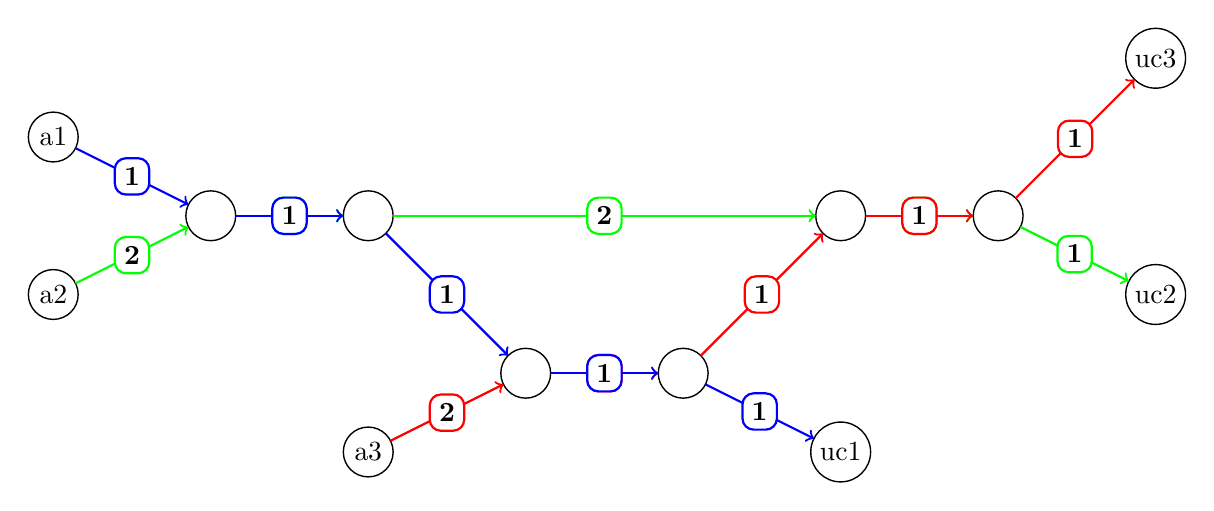
\begin{tikzpicture}
  \SetGraphUnit{5}
  \Vertex[x=4,y=2]{a3}
  \Vertex[x=0,y=4]{a2}
  \Vertex[x=0,y=6]{a1}
  
  \Vertex[x=14,y=7]{uc3}
  \Vertex[x=14,y=4]{uc2}
  \Vertex[x=10,y=2]{uc1}
  
  \SetVertexNoLabel
  \Vertex[x=2,y=5]{A}
  \Vertex[x=4,y=5]{B}
  \Vertex[x=10,y=5]{C}
  \Vertex[x=12,y=5]{D}
  \Vertex[x=6,y=3]{E}
  \Vertex[x=8,y=3]{F}
  \tikzset{
  EdgeStyle/.append style = {green} }
  \Edge[label = 2](a2)(A)
  \Edge[label = 1](A)(B)
  \Edge[label = 2](B)(C)
  \Edge[label = 1](C)(D)
  \Edge[label = 1](D)(uc2)

  
   \tikzset{
  EdgeStyle/.append style = {red} }
  \Edge[label = 2](a3)(E)
  \Edge[label = 1](E)(F)
  \Edge[label = 1](F)(C)
  \Edge[label = 1](C)(D)
  \Edge[label = 1](D)(uc3) 
     \tikzset{
  EdgeStyle/.append style = {blue} }
  \Edge[label = 1](a1)(A)
  \Edge[label = 1](A)(B)
  \Edge[label = 1](B)(E)
  \Edge[label = 1](E)(F)
  \Edge[label = 1](F)(uc1)

\end{tikzpicture}

\end{document}